\documentclass{article}
\usepackage{graphicx}
\usepackage{float}
\usepackage[utf8]{inputenc}
\usepackage{csquotes}
\usepackage{cleveref}
%\usepackage{biblatex}


\setlength{\parindent}{0cm} %Indenteringen för första raden på ett nytt stycke
\setlength{\parskip}{3mm} %Avståndet för en ny rad inom samma section
\setlength{\hoffset}{-40pt} % Flyttar vänstermarginalen -70
\setlength{\textwidth}{430pt}

\begin{document}
	
\pagenumbering{<command>}
\pagenumbering{Roman}
	
\title{Automatic Detection and Localization of Relatively Permanent Pigmented or Vascular Skin Marks}
\author{Armand Moulis}
\date{\today}
\maketitle

\newpage

\listoffigures

\listoftables

\newpage

\setcounter{tocdepth}{3}
\tableofcontents

\newpage

DETTA KOMMER ATT TAS BORT NÄR VÄL RAPPORTEN ÄR KLAR. KAN DOCK VARA AV INTRESSE UNDER TIDENS GÅNG 
\section*{Document history}
\begin{center}
	\begin{tabular}{|l|l| p{5cm} |l|l| }
		\hline
		Version & Date   & Changes & Sign & Reviewed \\ \hline
		0.1     & \today &         &      &  \\ \hline
	\end{tabular}
\end{center}


%% Start of the document

\section*{Abstract}

\textit{Keywords:} facial marks, 

\setcounter{page}{1}
\pagenumbering{arabic}
\newpage


\chapter{Introduction}\label{cha:intro}

Recently, the advancements in image analysis and computer vision provide many tools for forensics. One of the most promising tools are automated person identification which can help judicial system. The person identification are dependent on good facial features such as skin marks. This is the reason why this master thesis will investigate how to best detect and classify facial skin marks. 

\section{Background}

The work of systematically recording physical measurements for law enforcement was introduced by Alphonse Bertillon as early as in the 19th century. He developed the Bertillonage system since he believed that each person could be uniquely identified by a set of measurements \cite{Bertillon}. This system was however outdated quickly due to the rapid advancements in technology.

Today, the amount of video surveillance cameras, security cameras and cellphone cameras increases rapidly and there exist millions of devises capable of catching perpetrators in the act. The videos and still images can be used as evidence for identification during trials where forensic experts evaluate the strength of evidence whether if the suspect is the same person as the one caught
on camera.

One common method of evaluating whether the perpetrator and the suspect are the same person is to compare facial features such as eyes, nose, mouth, scars, and other facial marks. This is nowadays done manually \cite{face_soft} by the forensic examiners, and in order to evaluate the strength of the results, a likelihood ratio \cite{NFC_stat} from Bayes rule is calculated. The likelihood ratio is estimated from two hypotheses, where the numerator gives the probability to achieve the results if the perpetrator and the suspect are the same person. The denominator gives the probability to achieve the results if the perpetrator is another man. 

Facial features are divided into two groups: class and individual characteristics \cite{forensic_identification}. The class characteristics includes traits which put individuals into larger groups. Some of these feature are e.g. hair and eye colour, overall facial shape and size of the ears. The class characteristics does not suffice to identify unique individuals. Individual characteristics are traits that are unique to an individual, for example the number and location of facial skin marks.

Facial skin marks are any salient skin region that appears on the face. The most common facial marks are moles, pockmarks, freckles, scars, and acne. Some of these marks are not permanent, e.g. acne usually heals without leaving any permanent marks, while scares and moles remain the whole life \cite{automatic_detector_2015}. Skin marks which can be used for identification need to be relatively permanent, common and also be observable without any special imaging or medical equipment. These relatively permanent marks usually occur due to increased pigmentation or vascular proliferation. Therefore these kind of facial skin marks are called "relatively permanent pigmented or vascular skin marks (RPPVSM)". \cite{statistic_RPPVSM} 

This master thesis will separate facial skin marks into two classes: permanent and non-permanent facial marks. Some examples of the two types can be seen in \cref{fig:per_vs_non}. Which class a facial skin mark belong to is decided by the forensics forensics at National Forensic Centre (NFC) i Sweden. NFC is currently running a project where an automatic facial recognition system can be used to extract statistics from a database of facial images. The main advantages of using such a method are that the likelihood ratio can be calculated based on statistics, and that the risk for human bias in the decision process is diminished.

\FloatBarrier
\begin{figure}[h]
	\centering
	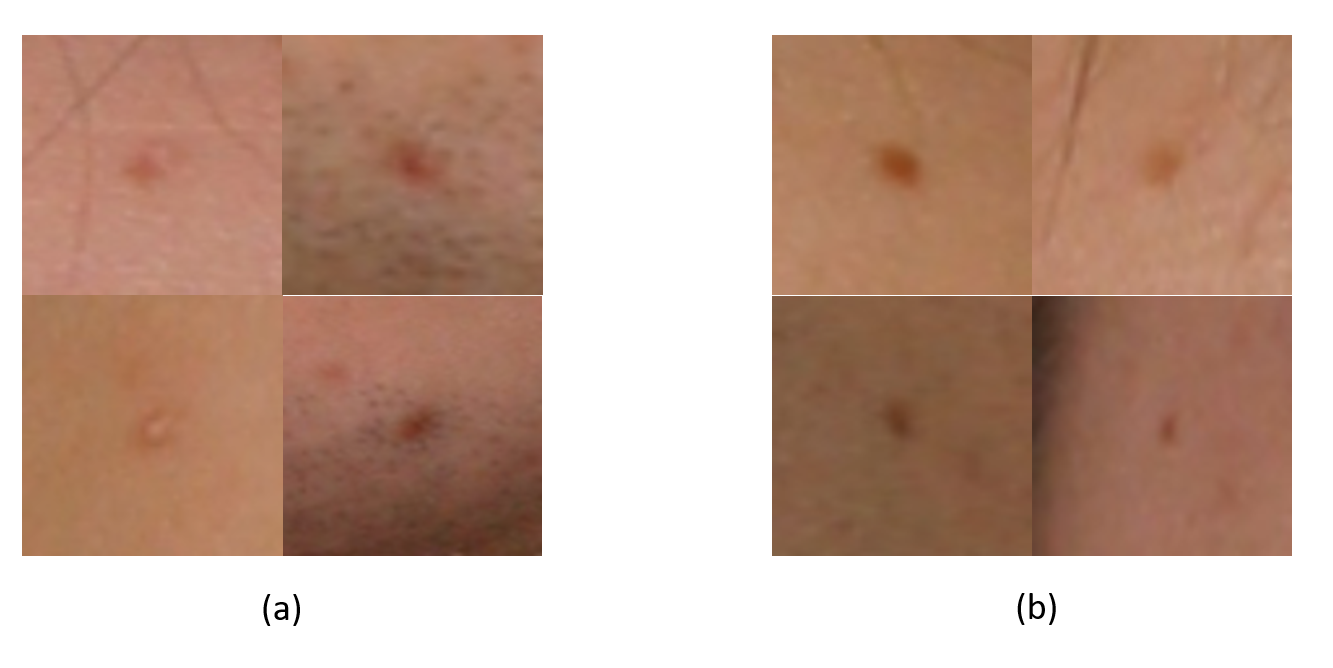
\includegraphics[width=\textwidth,height=\textheight,keepaspectratio]{per_vs_non}
	\caption{Examples of facials marks: (a) non-permanent, (b) permanent \label{fig:per_vs_non}}
\end{figure}
\FloatBarrier

This master thesis was started due to the need of combining the automatically calculated likelihood ratio value with the evidential value derived from the frequency of facial marks in certain regions of the face. The NFC is supporting this work by providing guidance and practical help.

\section{Related work}

A line of research relevant to this master thesis is the work by Vorder Bruegge et al. \cite{automatic_detector_2015} which proposed a fully automatic multiscale facial mark system. It detects facial marks which are stable across the the RGB-channels and different scales. These scales are called Gaussian pyramid and consist of low-pass filtered and subsampled images of the original image. This method to detect permanent marks are also used by Nisha Srinivas et al. \cite{twins} who tries to separate identical twins with an automatic multiscale facial mark detector. This method does not try to separate permanent and non-permanent facial mark rather tries to detect the more permanent marks.  

An other option considered when looking for facial marks are object detection and object classification.
The research on object detection and object classification is a wide and relevant field. Some of the things researchers have tried to detect and classify are faces \cite{facedetection_LBP}, pedestrians \cite{pedestrian_detection} and vehicles \cite{vehicle_hog}. These examples uses descriptive features based on histogram of oriented gradients (HOG) and local binary patterns (LBP). Face detectors also uses Haar-like features \cite{face_detection}. These three sets of features all describes the shape and structure of the searched object.

Taeg Sang Cho et al.\cite{reliable_mole} proposed a method using a Support Vector Machine (SVM) as a classifier to separate true and false mole candidates. They used a gist-descriptor as descriptive features. The gist-descriptor is designed to describe texture patterns over space. Read more about the gist-descriptor in the work of Antonio Torralba et al.\cite{gist_descriptor}. 

An other work using classifier are the work from Arfika Nurhudatiana et al. \cite{torso_RPPVSM}. They tried to detect and separate RPPVSM from non-RPPVSM on back torsos. They tried out three different classifiers which include a SVM, neural network and a binary decision tree. As input, the classifier was given the same set of features which included contrast, shape, size, texture, and color. Tim K. Lee et al.\cite{torso_mole} also used the same kind of features but does not use a trained classifier to separate true and false moles on back torsos. They use unsupervised algorithm to classify the mole candidates. 

When it comes to the detection of potential skin mark, there often involves some kind thresholding of a edge enhanced images. Using Laplacian of Gaussian (LoG) kernel as edge enhancement is popular method \cite{tattoos,face_matching}. After the edge enhancement of a image, the skin marks are highlighted and can then be segmented with different thresholding methods. 

\section{Motivation}

The work \cite{reliable_mole,torso_RPPVSM,torso_mole} all try to separate skin marks and they use a fixed set of features to do this. Arfika Nurhudatiana et al. compare different classifiers but there have been little work on comparing different set of features to separate permanent and non-permanent skin marks. This is why this thesis work will focus on comparing different features as input to a supervised classier. Since the facial marks have a circular shape and mostly vary in color it would bee wise to use colors maps as features. 

This master thesis will look at a recently used and interesting method to highlight the skin marks, instead of the common LoG kernel. The algorithm is called fast radial symmetry (FRS) \cite{twins,automatic_detector_2015} and it highlights radially symmetrical regions and suppresses regions that are asymmetrical. This is ideal when one is looking for circular objects which is perfect since facial marks are often circular. The FRS is expected to be more suitable for detecting skin marks compared to previous approaches, and is therefore investigated in this thesis.

The challenge with detecting skin marks, especially in the face, is that there are many other structures which can be mistaken as facial marks, e.g. nostrils, facial hair. Facial hair in the form of stubble can complicate the problems, as its appearance may be similar to a facial mark. The main challenge of this work is to find characteristic features for the permanent and non-permanent skin marks. They differ little in shape and structure but differ more in color. This master thesis will try to overcome these challenges. 


\section{Aim}

The aim of thie master thesis is to develop a method for creating a large data base with facial images and the location of facial marks. Such a database would provide better statistics for the evidential value in forensic facial image comparison examinations. The algorithm should detect facial marks automatically from a color image and then separate them into a permanent and non-permanent group.

\section{Problem specification}

From a single facial RGB-image en face, facial marks should be detected and classified as a permanent or non-permanent mark. This task can be divided into five smaller tasks. These task will be described more in detail in later chapters.

\textbf{\textit{Task 1: Pre-processing}}
The image can be illuminated unevenly and rotated which can cause difficulties when detection potential facial marks. Thus, the image has to be geometrically and photometrically normalized. 

\textbf{\textit{Task 2: Candidate detection}}
The actual detection of potential marks are done with the help of radial symmetry in the image. The algorithm will search for areas which contains edges that have a circular shape.   

\textbf{\textit{Task 3: Post-processing}}
Among the potential facial marks, there can be many false detections such as nostrils, facial hair, pupils et cetera. The false detection has to be eliminated and will be done with a hair removal method, blob identifier, size eliminator and face segmentation.

\textbf{\textit{Task 4: Classification}}
When the marks has been detected, they have to be sorted into the two classes, permanent and non-permanent. This is done by calculating different descriptive features. These features is used to train a supervised support vector machine. With the trained classifier, the facial mark can sorted. 

\textbf{\textit{Task 5: Feature selection}}
The major task in this master thesis is to compare and evaluate different descriptive features. This is done by choosing different sets of features for the classifier and evaluate the performance of the classifier for each set. 

\section{Scope}

In general, when working with image, the quality of the images are crucial for the results. Low resolution and badly illuminated images taken from different angles can cause analytical difficulties. Therefore, this thesis assumes images which are high resolute, well illuminated, taken en face and in RGB-colours. 

Also, this master thesis will focus on a comparison between different sets of features for the classifier instead of examining different ways of detecting facial marks. This is due to the little work done regarding feature selection. 

The classifier will only be a binary classifier because no non-facial marks has been collected as labelled data during the thesis work due to lack of resources.   

\section{Thesis outline}

This chapter describes the aim and problem specification of this master thesis. In Chapter \ref{cha:theory}, gives an insight in theory behind the methods used in the algorithm. Chapter \ref{cha:method} describes the pipeline of the algorithm and the implementation of the theory used in it. The results from the algorithm can be studied in Chapter \ref{cha:result} and an discussion about the result and methods used is found in Chapter \ref{cha:Discussion}. Finally, Chapter \ref{cha:conclusion} consist of a conclusion of the master thesis and ideas for future work within the same scope. 

\chapter{Related work/Background }
The work of systematically recording physical measurements for law enforcement was introduced by Alphonse Bertillon as early as in the 19th century. He developed the Bertillonage system since he believed that each person could be uniquely identified by a set of measurements \cite{Bertillon}. This system was however outdated quickly thanks to the explosion of technology.

Resent research by Srinivas et al. \cite{automatic_detector_2015} have resulted in an automatic and semi-automatic facial recognition processes. It uses a multiscale automatic facial mark detector for the automatic detector and receive a equal error rate of 15.48\%. This result was improved by introducing human knowledge in the semi-automatic detector.

When distinguishing identical twins it is useful to look at facial marks which has been examined in an other article by Srinivas et al. \cite{twins}. The study concluded that the facial marks can be uses as features for distinguishing between identical twins even if there seems to exist a correlations between the twins set of marks.

Nurhudatiana et al. \cite{statistic_RPPVSM} describes in their article the distribution of Relatively Permanent Pigmented or Vascular Skin Marks (RPPVSM) in Caucasians, Asians, and Latinos. They conclude that if the number of RPPVSM are few they are randomly distributed which can be used for personal identification in law enforcement. 

Anil and Park found during their research \cite{jain_facial} that facial mark can be used to increase the recall and precision for a state-of-the-art face matcher (FaceVACS). The facial mark detector used the 3x3 LoG-operator as blob detector. Adding these features to the algorithm improved the face matcher from  92.96\% to 93.90\% on the Facial Recognition Technology (FERET) database and from 91.88\% to 93.14\% on a Mugshot face database. 




\section{Facial marks}
The skin in the face does not have a homogeneous colour and contains regions with different coloured facial marks. The most common facial marks are moles, pockmarks, freckles, scars, and acne. Some of these marks are not permanent, e.g. acne usually heals without leaving any marks, while scares and moles remain the whole life    \cite{automatic_detector_2015}. Skin marks which can be used for identification are called RPPVSM and they have to be relatively permanent, common and also be observable without any special equipment. \cite{statistic_RPPVSM}

\chapter{Method}\label{cha:method}

This chapter will describe the pipeline of the algorithm developed during this master thesis. The different parts of the algorithm are viewed with a more implementation focused view.

\section{Overview}

An overview of the algorithm is presented in figure \ref{fig:detection_flow}. The algorithm start of with pre-processing an input image. This step makes sure that the image is normalized and that all necessary sub-parts are generated. Then a facial mask is generated in the segmentation step. Now the algorithm have everything in order to detect the skin mark candidates. All the candidates are then post-processed to eliminate false detections. Finally, the remaining skin marks are classified as a permanent or non-permanent skin mark.    

\FloatBarrier
 \begin{figure}[h]
 	\centering
 	
\includegraphics[width=\textwidth,height=\textheight,keepaspectratio]{flow_report}
 	\caption{Overview of the algorithm \label{fig:detection_flow}}
 \end{figure}
\FloatBarrier

\section{Data and annotation}

To evaluate the algorithm, a set of 106 images of faces en face were acquired from SCface database \cite{SCface} and FRGC database \cite{FRGC}. These images where collected at University of Zagreb and University of Notre Dame respectively. The purpose of the databases is to provide data to develop and improve face recognition algorithms. The images where taken in under controlled conditions indoor in a studio setting indoor with a high-quality photo camera. Figure \ref{fig:orig_img} shows an example of the images from the databases.

\FloatBarrier
\begin{figure}[h]
	\centering
	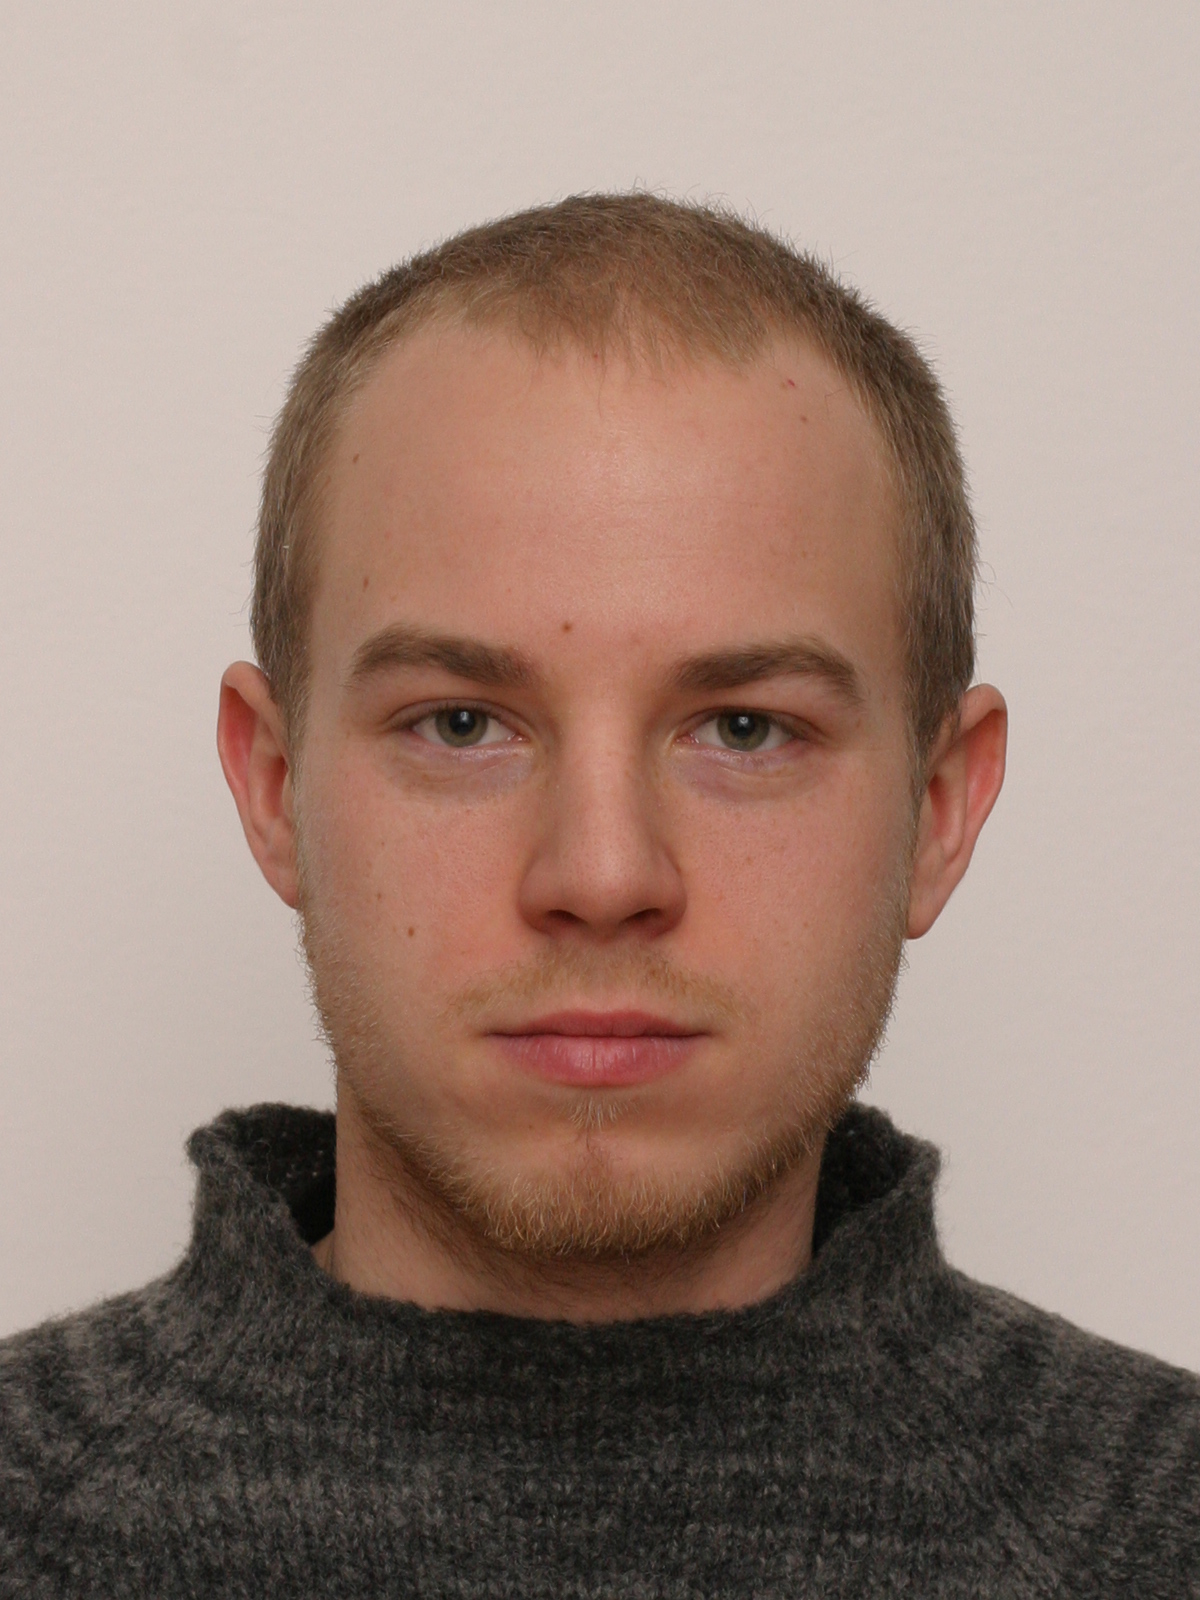
\includegraphics[width=\textwidth/2,height=\textheight/2,keepaspectratio]{001_orig}
	\caption{One example of the images used to evaluate the algorithm \label{fig:orig_img}}
\end{figure}
\FloatBarrier

Each image was examined the supervisors at NFC who labeled facial skin mark of interest. Each mark was given either the label permanent or non-permanent according to NFC definitions. This resulted in 506 marks where 353 were labeled as permanent and 153 non-permanent. 

\section{Pre-processing}

When the algorithm is given a RGB image, denoted $I$, it first detects the location of the face with the help of the face detector in OpenCV. It surrounds the face with a bounding box. With the bounding box, the facial landmarks can be detected by using the algorithm from Dlib. This landmark algorithm was chosen since it converges faster than other state of the art methods \cite{dlib_landmark}. 

\FloatBarrier
\begin{figure}[!h]
	\centering
	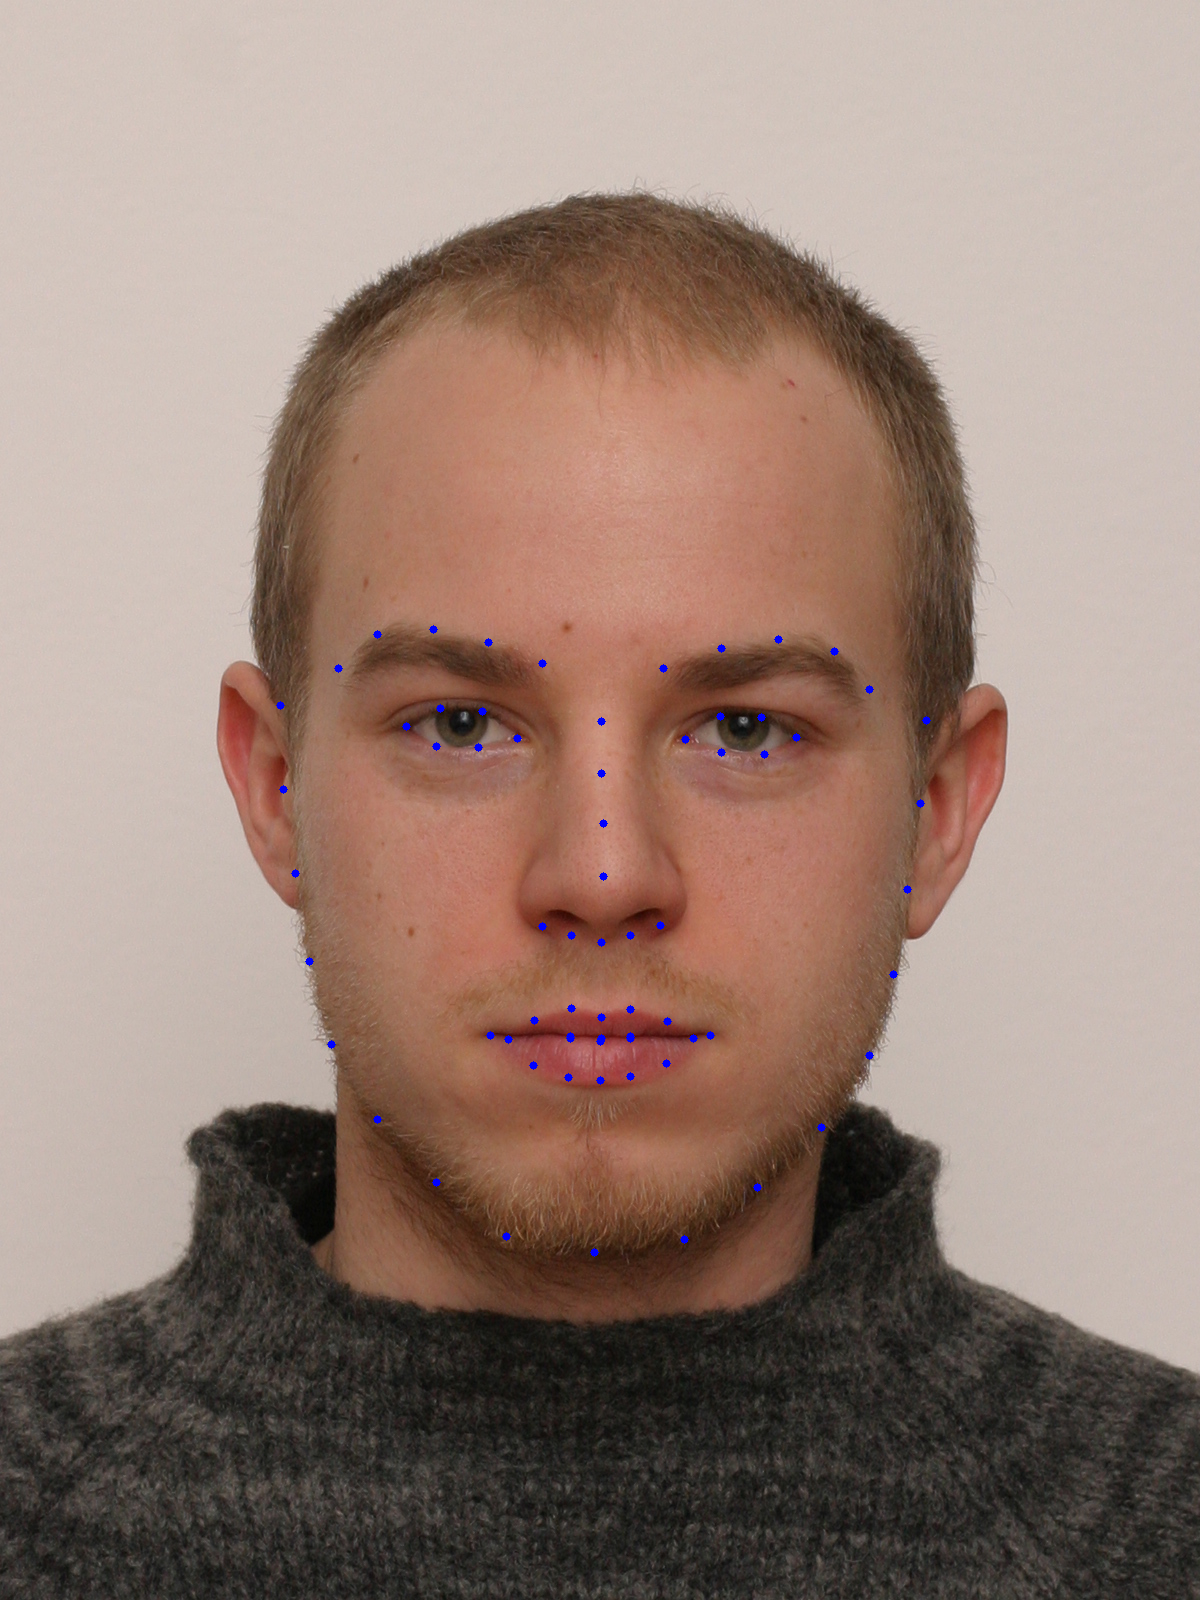
\includegraphics[width=\textwidth/2,height=\textheight/2,keepaspectratio]{landmarks}
	\caption{Image with the 64 landmarks shown as blue dots \label{fig:landmarks}}
\end{figure}
\FloatBarrier

With the landmarks, it is possible to begin the normalization process, see \cref{sec:normalization}. First, the image is photometric normalized using LRSR algorithm. This tone mapping operator is fast and had a good implementation available in C++. It performs on pair with the best tone mapping operator of today \cite{badger}. Photometric normalization is vital since the visibility of facial marks can be affected by varying illumination of the image.  

Second, the image is rescaled such that the interpupillary distance is 500 pixels. This resizes the images to approximately 2100x2800 and the interpolation method used is cubic interpolation. The landmarks are also used to rotate the image so that the eyes are level. The rotation and resizing of the image is called geometric normalization and is necessary remove the effect of the distance and tilt of the camera. In \cref{fig:rotated_img} one can see the result from the image normalization. 

\FloatBarrier
\begin{figure}[!h]
	\centering
	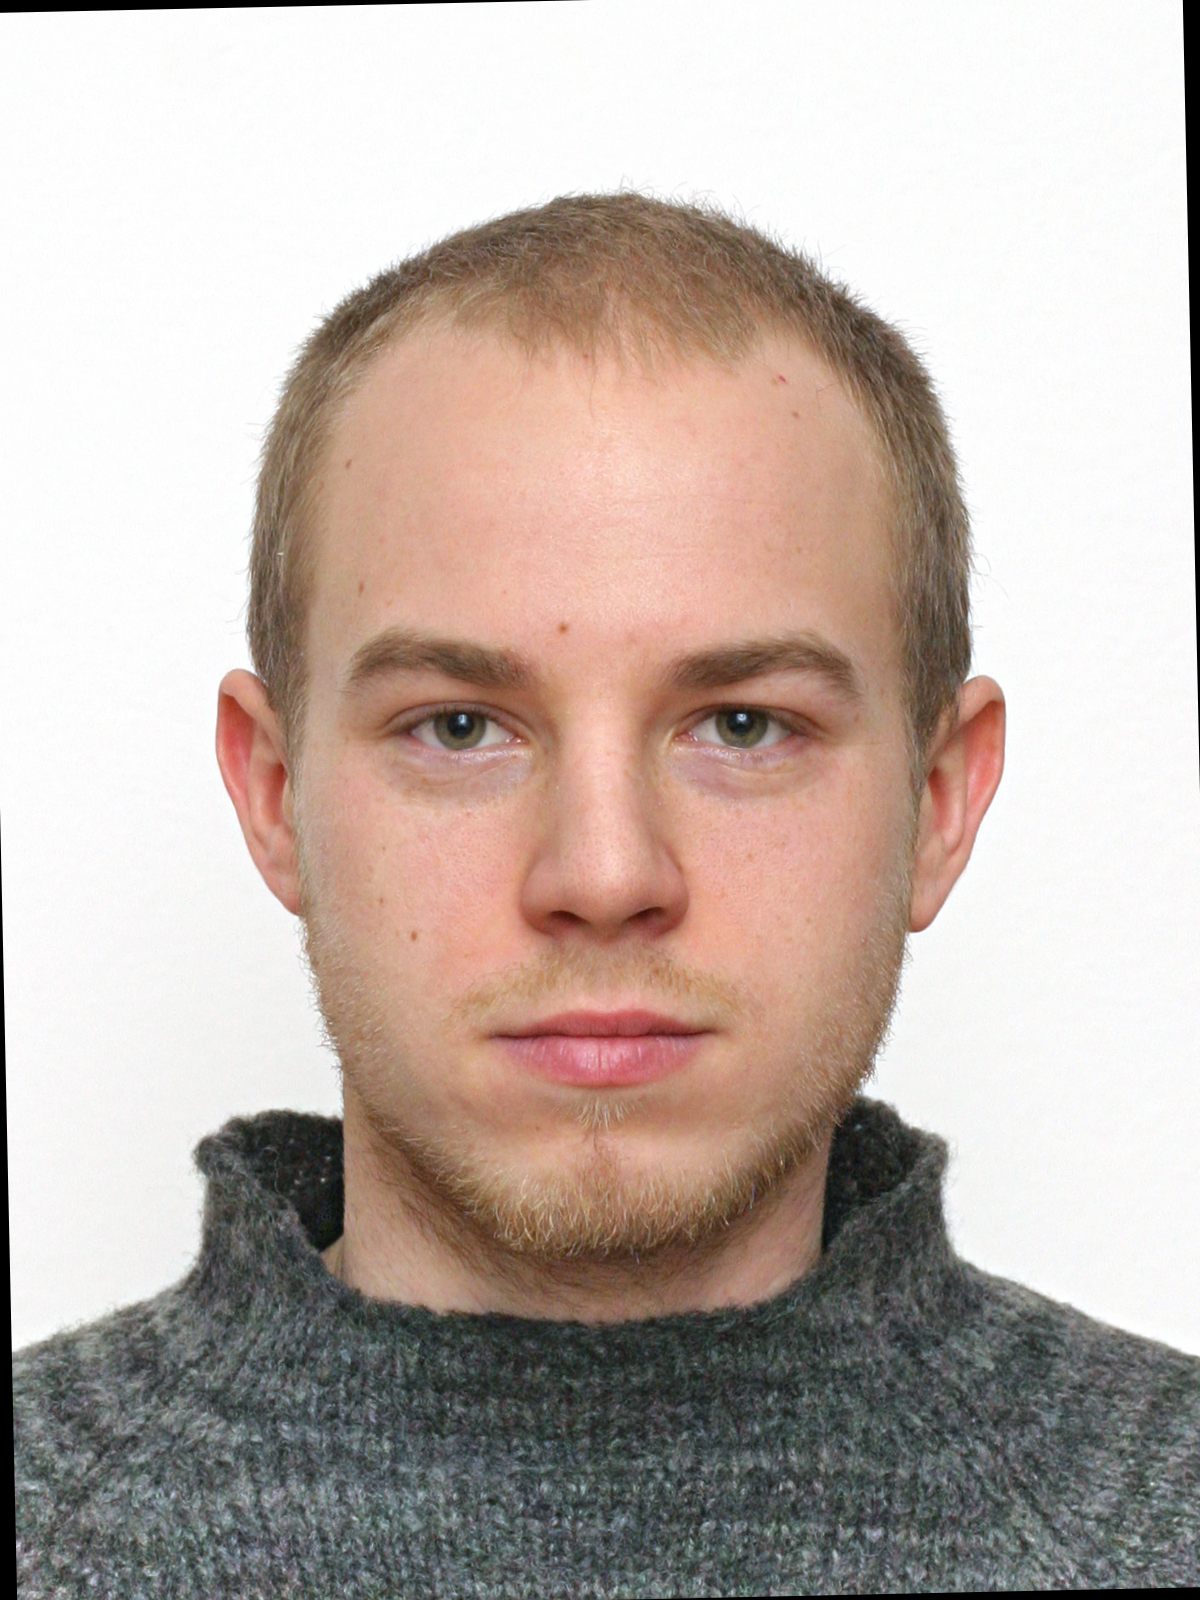
\includegraphics[width=\textwidth/2,height=\textheight/2,keepaspectratio]{001_rotated}
	\caption{Image after photometric and geometric normalization \label{fig:rotated_img}}
\end{figure}
\FloatBarrier

The last part of the pre-processing step is to segment out areas, see \cref{sec:segmentation}, which can cause false detections such as facial hair, nostrils, pupils etc. This is done by generating a binary mask. To segment out areas with skin, the implementation of GrabCut in OpenCV was used since it has proven to perform as well or better than many other user interactive foreground extraction methods \cite{grabcut}. From the skin mask, the eyes, nostrils, mouth and throat are cut out using elliptical shapes around the landmarks marking these regions. To expand these holes, a morphological erosion algorithm was performed on the image with a 3x3-kernel containing ones. The resulting mask can be observed in \cref{fig:mask_img}. 

\FloatBarrier
\begin{figure}[!h]
	\centering
	
\includegraphics[width=\textwidth/2,height=\textheight/2,keepaspectratio]{001_mask}
	\caption{Image of the facial mask \label{fig:mask_img}}
\end{figure}
\FloatBarrier        

\section{Candidate detection}

The pre-processed image, denoted $I_{pre}$, can now be used to search for facial skin mark candidates. This is done with the help of FRS algorithm, see \cref{sec:FRS}. It highlights circular shapes which can be more easily detected. The algorithm makes calculations with different radii, $N$, and the ones used are $N = \{1, 3, 5, 7, 9, 11, 13, 15 \}$. These radii were used since 75\% of facial marks had an area smaller than 600 pixels, see \cref{fig:result_box_size}. The Gaussian kernel $A_n$ size increased from 3x3 to 7x7 depending on the radius $r$. 

Below, \cref{fig:frs}, the resulting FRS image is presented. It is hard to see the facial marks since the image contains positive and negative values. By taking the absolute value of the image, the marks appear more prominent, see \cref{fig:frs_abs}.  

\FloatBarrier
\begin{figure}[h]
	\centering
	\includegraphics[width=\textwidth/2,height=\textheight/2,keepaspectratio]{frs}
	\caption{FRS image \label{fig:frs}}
\end{figure}
\FloatBarrier

\FloatBarrier
\begin{figure}[h]
	\centering
	\includegraphics[width=\textwidth/2,height=\textheight/2,keepaspectratio]{frs_abs}
	\caption{Absolute value of FRS image \label{fig:frs_abs}}
\end{figure}
\FloatBarrier

At this point, an FRS-image with points of interest has been acquired. From this image, a binary threshold was applied with the threshold $h_{FRS}$, see \cref{eq:bin_thresh}.

\begin{equation} \label{eq:bin_thresh}
I(p) = 
\begin{cases}
1    & \quad \text{if } I(p) \geq h_{FRS} \: \text{max}(I) \\
0		& \quad  \text{ else}\\
\end{cases}
\end{equation}

This results in a binary image which is used in the watershed algorithm described by Fernand Meyer \cite{watershed}. The use of watershed is good since it can find the contour of uneven marks as long as the pixels approximately have the same intensity value. The watershed algorithm is applied on a gray image of the face. The output from this is a set of bonding boxes containing facial marks candidates.

The $h_{FRS}$ is the only parameter which is varied in the candidate detector. It is varied to examine the performance of the detector by looking at the recall and precision value of the detector. 

\section{Post-processing}

After candidate detection, the false detection was eliminated by using three methods. The first method finds candidates which contains a blob. The blob detector in OpenCV was used and it was given the three parameters: inertiaRatio, convexity and circularity. The method also allows to sort out all candidates which contains more than one blob. These candidates was eliminated. 

%minInertiaRatio = 0 vs 1
%minconvexity = 0 vs 1
%minCircularit = 0 vs 1

The second part removes candidates which contain to many hair pixels. The $h_{hair}$ threshold, see \cref{subsec:hair_eli}, was set to 0.02 and candidates containing more than 10\% hair pixels was excluded.

The parameters from the first and second eliminator was chosen such that the number of false detection was reduced while preserving true detections. This was done by examining a few images with different parameter settings. 

The third and last method simply removed all candidates which had a larger area than 1000 pixels. This value was chosen since no annotated marks had a area larger than that, see \cref{fig:result_box_size}. 

\section{Classification}

When a set of facial marks has been acquired through the skin mark detector, they have to be separated into permanent and non-permanent marks. This is done with a non-linear SVM with a RBF-kernel, see \cref{sec:machine_learning}. It was trained with different sets of feature descriptors, \cref{table:feature_sets}. Each set was trained with one part training data and evaluated with one part of test data.

The parameters $C$ and $\gamma$ was optimized by first training the classifier with a crude range of values. The $C$-value and $\gamma$ that gave the best accuracy from the crude grid of values was located. Next a finer grid search was performed in the region of the best pair of $C$ and $\gamma$. From this finer grid, the best parameters for the specific set of features could be picked out. Each grid of parameters contained 20x20 pair of parameters. The low number of pairs was chosen to reduce the computation time when searching for the best parameter pair.  

When in comes to the feature descriptors, see \cref{sec:features}, the LBP-features has no variable parameters which is used in this master thesis. The HOG-features needs a couple of parameters. The window size was set to 48x48 pixels, block size was 8x8, block stride was 4x4, cell size 4x4 and 9 bins. 

The different set of features used to train the classifier can be seen in \cref{table:feature_sets}. Here, COLOR means the 11 color names described in \cref{subsection:Color}. 

\FloatBarrier
\begin{table}[h!]
	\begin{center}
		\caption{Sets of feature descriptors to be evaluated}
		\begin{tabular}{|c|l|}
			\hline
			Set &  Features   \\ \hline
			 1  &     RGB     \\ \hline
			 2  &     HSV     \\ \hline
			 3  &    COLOR    \\ \hline
			 4  &     HOG     \\ \hline
			 5  &     LBP     \\ \hline
			 6  &  HOG + RGB  \\ \hline
			 7  &  HOG + HSV  \\ \hline
			 8  & HOG + COLOR \\ \hline
			 9  &  LBP + RGB  \\ \hline
			 10  &  LBP + HSV  \\ \hline
			 11  & LBP + COLOR \\ \hline
			 12  & RGB + HSV + COLOR \\ \hline
		\end{tabular}
		\label{table:feature_sets}
	\end{center}
\end{table}
\FloatBarrier

\section{Implementation details}

The algorithm was implemented in Visual Studio 2013 using the OpenCV 3.0.0 \cite{opencv} for most image processing. The landmark detection algorithm comes from an open source library Dlib 18.18 \cite{dlib09}. When it comes to the graphs and bar-diagrams in this master thesis, Matlab \cite{MATLAB:2010} was used since it is easy to produce good looking graphs.  

%To evaluate the detector and classifier, the performance values recall, precision and accuracy was used. For the detector, recall and precision was used to compare the performance of the $h_{FRS}$-value and the different elimination methods. For the classifier the accuracy measurement was used. A five-fold cross validation was used throughout the evaluation of the classifier.   






























%\subsection{Facial grid}
%
%The landmarks are also used to produce a grid over the face. The grid consist of 16 regions which are defined the supervisors at NFC. This grid is needed to calculate the number of facial marks within these predefined regions. This is necessary to improve the evidential value of the likelihood ratio.
%
%\begin{figure}[h!]
%	\centering
%	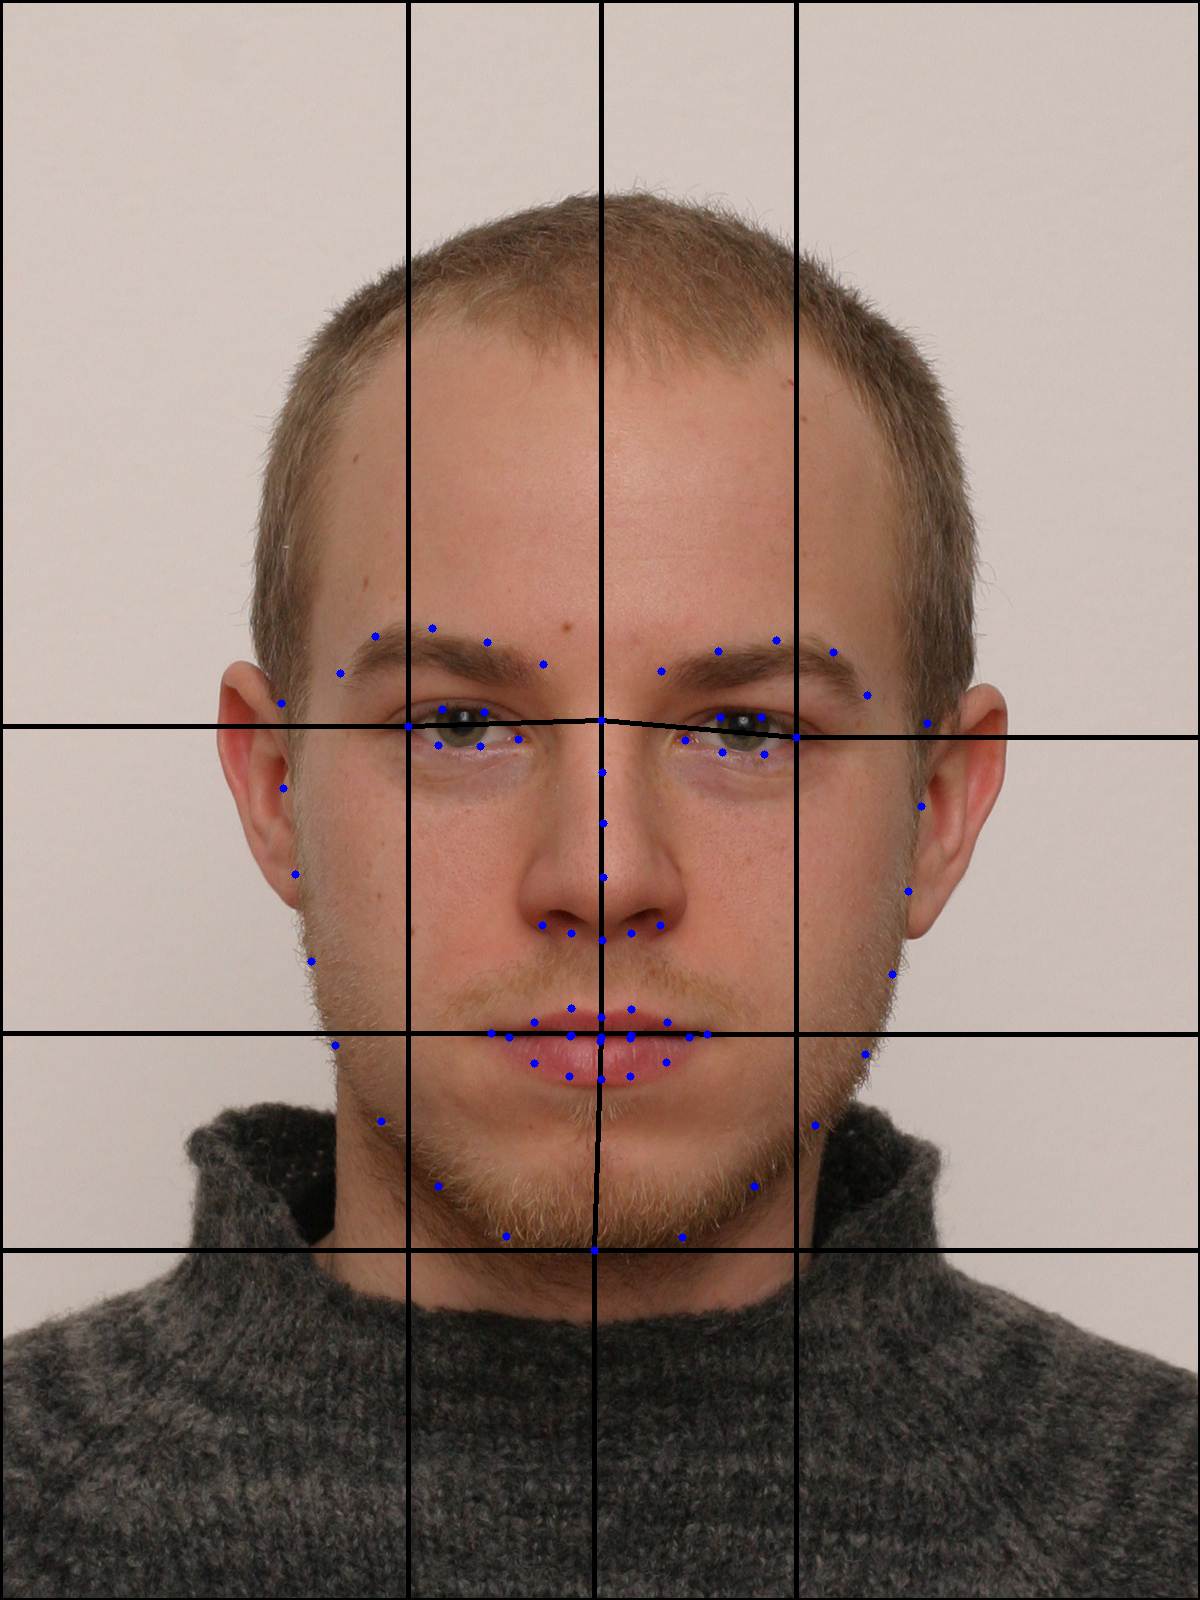
\includegraphics[width=\textwidth/2,height=\textheight/2,keepaspectratio]{001_grid}
%	\caption{Image over the landmarks (blue points) and facial grid (black lines) \label{fig:grid_img}}
%\end{figure}
%
%\section{Classification}
%
% Generally, support vector machine (SVM) tend to perform better with continuous and multidimensional features and with a large amount of samples. The features used in this case fulfill the continuity and multi dimension. Chih-Wei et. al. \cite{svm_guide} also describes a good way to optimize the use of SVM and recommend to use radial basis function (RBF) as kernel. This is why a SVM with RBF kernel is chosen for the mark classifier.  
%
%The goal with a SVM is to separate different classes by finding the best hyperplane which divides them. The hyperplane is moved such that a loss-function is minimized. RBF kernel nonlinearly maps samples into a higher dimensional space which allows the classifier to handle non-linearly separable classes. This kernel also has fewer numerical difficulties. The parameters needed for a RBF kernel i $C$ which determines the penalty parameter for the error and $\gamma$ which defines how far the influence of a single training sample reaches. \cite{svm_guide}
%
%The training data consists of the labelled facial marks provided by the supervisors at NFC. To get a good classifier, a set of discriminative features are required.
%
%\subsection{Features}
%
%The most common color space in use is the RGB system, one channel each for the red, green and blue colors. Arfika Nurhudatiana et al. \cite{torso_RPPVSM} used, among others, the minimum, maximum, and average from the RGB-channels as discriminative features. 
%
%The features extracted from the facial marks are the mean and the standard deviation from the three RGB channels and the 11 colours from the work of Joost van de Weijer et al. This results in 28 features which is used to train the classifier. 
%
%To not let some feature with greater numeric rang dominate over features with smaller range, the features need to be scaled \cite{svm_guide}. This is very important which is why the features are linearly scaled to a range from $0$ to $1$. The same scaling factor has to be used when the test data is scaled. 






  

\chapter{Result}\label{cha:result}

This Chapter first describes the experiment to evaluate the algorithm and then presents the results.

\section{Experiment}

The experiment was set such that the image set was processed by the algorithm with 11 different thresholds values, $h_{FRS}$, for the FRS-image. The $h_{FRS}$ ranged from $0.05$ to $0.15$. The output was compared to the ground truth. A correct detection was defined as all detections which had a union with an annotated mark. This definition has been chosen since some of the detections can be very small. Also, since candidates larger than 1000 pixels has been eliminated, no overly large candidates can give correct detections.   

The $h_{FRS}$-value which gives the best recall value was used to evaluate the elimination process of the candidates. This was done by calculating the precision and recall values before the different elimination steps. The results is displayed in \cref{fig:results_bar_frs}.

To evaluate how the elimination process is working, the recall and precision values after each elimination step. These results can be observed in \cref{fig:results_bar_elimniation}.

To evaluate the facial mark classifier, a cross validation of the 506 annotated mark were performed. 100 marks was chosen at random to be used as test marks while the remaining marks was used for training the SVM. This was repeated until all the marks had been used as test marks.

In order to find the best set of descriptive features from \cref{table:feature_sets}, the classifier was trained for each set of features. The parameters $C$ and $\gamma$ was optimized for each set.  

%In order to find the best $C$-value and $\gamma$-value for the mark classifier, the parameters are varied over a rough interval to narrow down the search. Afterwards, a more fine interval is used to find the best parameters. This has been shown by Chih-Wei et. al. \cite{svm_guide}  to be an effective method compared to a more random selection of parameters which is often used by people unfamiliar to SVM. 

\section{Results from experiment}

This section will present the results from experiment described above. The result is divided into two parts: Detector and Classifier. 

\subsection{Detector}

Here the results from the facial mark detector is presented. In the \cref{fig:results_bar_frs}, the precision and recall for different $h_{FRS}$-value can be examined. The precision corresponds to the white bar and the recall corresponds to the black bar. Note that this is only the detections of facial mark and no classification between permanent and non-permanent marks. 

\FloatBarrier
\begin{figure}[h!]
	\centering
	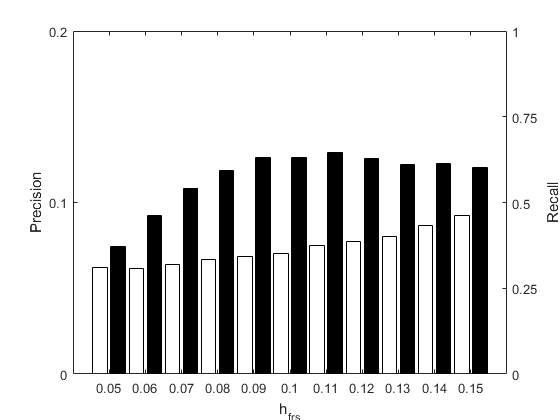
\includegraphics[width=\textwidth*3/4,height=\textheight*3/4,keepaspectratio]{results_bar_frs}
	\caption{Detection results from the algorithm with different $h_{frs}$-values. The white bars represent the precision value and the black bars represent recall value.  \label{fig:results_bar_frs}}
\end{figure}
\FloatBarrier

As one can see, the precision increases with higher $h_{FRS}$-value without affecting the recall substantially. This is means that the number of candidates decreases with a growing $h_{FRS}$-value. Thus, a small $h_{FRS}$-value results in a large amount of candidates while a larger value gives fewer candidates.

In \cref{fig:results_bar_elimniation}, it is possible to see the effects of the different elimination steps. As before, the white bar represent the precision and the black bar represent the recall. The first pair is the result just after the candidate detection and the second pair is the result after the blob detector. Furthermore, the third pair is after the hair eliminator and the last pair is after the size eliminator. 

\FloatBarrier
\begin{figure}[h!]
	\centering
	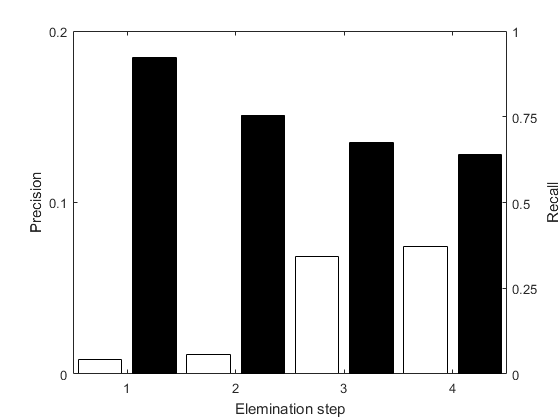
\includegraphics[width=\textwidth*3/4,height=\textheight*3/4,keepaspectratio]{results_bar_elimniation}
	\caption{Detection results from the algorithm  after different candidate elimination steps. 1 = before elimination, 2 = after blob-elimination, 3 = after hair-elimination, 4 = after size-elimination. The white bars represent the precision value and the black bars represent recall value.  \label{fig:results_bar_elimniation}}
\end{figure}
\FloatBarrier

It is obvious that the different eliminators are essential for the algorithm. The hair eliminator improves the precision the most while the blob detector worsen the recall the most.     


In \cref{fig:all_detections} below one can observe all the candidates found by the detector before post-processing. The candidates are shown as blue bounding boxes and the annotated facial marks for this image is show as red bounding boxes. There are many false detections in the hair and the beard which is some of the problems identified in this master thesis. 

After the post-processing, \cref{fig:all_hits}, almost all the false detection has been eliminated but some of them remain. The remaining false detection are located in the beard and hair. Some bounding boxes are around skin marks which has not been deemed of interest by the forensics at NFC. 

\FloatBarrier
\begin{figure}[h]
	\centering
	\includegraphics[width=\textwidth*4/10,height=\textheight*4/10,keepaspectratio]{001_all_detections}
	\caption{An image of all potential facial marks. Each potential mark is shown as a blue box and all annotated facial mark is shown as a red box. \label{fig:all_detections}}
\end{figure}
\FloatBarrier

\FloatBarrier
\begin{figure}[h]
	\centering
	\includegraphics[width=\textwidth*4/10,height=\textheight*4/10,keepaspectratio]{001_hits}
	\caption{An image of the final result of the detector. Green boxes denotes true detections, red boxes denotes annotated marks and blue boxes denotes false detections. \label{fig:all_hits}}
\end{figure}
\FloatBarrier

\subsection{Classifier}

Here the results from the different feature sets for the classifier is presented. When looking at the different features separately, \cref{table:single_feature}, one can see that the HOG and LBP feature perform bad compared to the color based features. 

\FloatBarrier
\begin{table}[h!]
\begin{center}
	\caption{Confusion matrix for single features}
	\begin{tabular}{|c|c|c|c|c|c|c|c|c|}
		\hline
		Feature set &  RGB  &  HSV  & COLOR &  HOG  &  LBP    \\ \hline
		    TP      &  336  &  334  &  335  &  348  &  313    \\ \hline
		    TN      &  107  &  104  &  107  &  32   &  88     \\ \hline
		    FP      &  17   &  19   &  18   &   5   &  40     \\ \hline
		    FN      &  46   &  49   &  46   &  121  &  65     \\ \hline
		 Accuracy   & 87,55 & 86,56 & 87,35 & 79,25 & 75,10   \\ \hline
	\end{tabular}
\label{table:single_feature}
\end{center}
\end{table}
\FloatBarrier

Now, if the color based features are added to the HOG and LBP features respectably, \cref{table:hog_features,table:lbp_features} it is clear that the color based features improve the accuracy for the structure based features. However, it is clear that the color names gives the best result to the classifier. 

\FloatBarrier
\begin{table}[h!]
	\begin{center}
		\caption{Confusion matrix for HOG and color based features}
		\begin{tabular}{|c|c|c|c|}
			\hline
			Feature set & HOG + RGB & HOG + HSV & HOG + COLOR \\ \hline
			    TP      &    326    &    341    &     332     \\ \hline
			    TN      &    63     &    46     &     111     \\ \hline
			    FP      &    27     &    12     &     21      \\ \hline
			    FN      &    90     &    107    &     42      \\ \hline
			 Accuracy   &   76,88   &   76,48   &    87,55    \\ \hline
		\end{tabular}
		
		\label{table:hog_features}
	\end{center}
\end{table}
\FloatBarrier

\FloatBarrier
\begin{table}[h!]
	\begin{center}
		\caption{Confusion matrix for LBP and color based features}
		\begin{tabular}{|c|c|c|c|}
			\hline
			Feature set & LBP + RGB & LBP + HSV & LBP + COLOR   \\ \hline
			    TP      &    313    &    313    &     333       \\ \hline
			    TN      &    89     &    88     &     106       \\ \hline
			    FP      &    40     &    40     &     20        \\ \hline
			    FN      &    64     &    65     &     47        \\ \hline
			 Accuracy   &   79,45   &   79,25   &    86,76      \\ \hline
		\end{tabular}
		\label{table:lbp_features}
	\end{center}
\end{table}
\FloatBarrier

If on combines the color based features \cref{table:color_features} the accuracy does not improve but stays at the same level as only using the color names. 

\FloatBarrier
\begin{table}[h!]
	\begin{center}
		\caption{Confusion matrix for color based features combined}
		\begin{tabular}{|c|c|}
			\hline
			Feature set & RGB + HSV + COLOR \\ \hline
			    TP      &    336    \\ \hline
			    TN      &    106     \\ \hline
			    FP      &    17     \\ \hline
			    FN      &    47     \\ \hline
			 Accuracy   &   87,35   \\ \hline
		\end{tabular}
		
		\label{table:color_features}
	\end{center}
\end{table}
\FloatBarrier

If one is interested how the accuracy changes depending on the parameters $C$ and $\gamma$, please look in the appendix. 







\chapter{Discussion}\label{cha:Discussion}

This section will discuss the results from the algorithm and the methods used to implement it. This section will also suggest future work and mention ethical perspective.  

\section{Result}

As seen, the detector has problem with false detections which is a huge problem. The precision is not very good, not even over 10\%, due to the many false detections. The precision does not increase faster than the decline of the recall with an increasing $h_{frs}$-value. This indicates that there are margins for improvement when it comes to the candidate detector.

Vorder Bruegge et al. \cite{automatic_detector_2015} got a precision of 71\% which is a lot better than the result from this master thesis. Taeg Sang Cho et al.\cite{reliable_mole} got a recall value of 84.7\% which is also better than the results from this master thesis. One thing that should be noticed is that Vorder Bruegge et al. has been focusing to finding RPPVSM which is a wide definition of skin marks. This master thesis has tried to find the skin marks which has been of interest to the forensics at NFC. This could be one of the reasons to the large amount of false detections. The detector is probably detecting RPPVSM which has not been deemed of interest.     

When looking at the elimination method used, they do improve the precision and recall values but maybe not to the extant which one was hoping for. There can be a great improvement in trying to find a optimal value for the $h_{hair}$ threshold since this has not be investigated. Maybe there are better methods to bee used to eliminate the false detections than the ones used in this master thesis.  

The classifier offers some indication to the importance of colors when it comes to separating permanent and non-permanent marks. The structural features alone perform all right but they do not improve the accuracy when they are combined with color based features. Simply put, they do not show complementary properties. 

The reason why the color based features perform better is probably due to the small differences in structure between permanent and non-permanent skin marks, see \cref{fig:per_vs_non}. One can see a slight difference in color, the permanent marks tend to be browner while the non-permanent marks tend to be more red.  

It is hard to compare the performance of the classifier with other research since researchers using classifiers for face recognition mostly use the classifier to find matching set of skin marks. For example, a classifier is used to determine if a set of skin marks matches other set of skin marks. Also, Taeg Sang Cho et al. used classifiers to find moles but they only tried to separate moles and everything else. This should be easier than separating permanent and non-permanent skin marks. In other words, this master thesis has looked at a more difficult problem which is why it is hard to compare the results from this master thesis with other research. 


\section{Method}

There are a lot to say about the methods used in the algorithm. The major problem with the algorithm is the elimination of candidates. They eliminate candidates which are true facial marks. The hair elimination part does improve the precision the best. The blob detector on the other hand is hardly improving the precision at the cost of recall loss. This means that the blob-detector is not contributing to the algorithm in a positive way.

Tim Lee et al. describes their algorithm well except when they are explaining how to calculate the hair mask for each color channel. It is not clear what the maximum from refers to. The algorithm in this work used the maximal pixel value between the different structuring elements. 

The mark detector used in the algorithm was good at indicating the potential facial marks but the simple thresholding method to pin point them out was not optimal. It kept the pixels larger than a certain percent of the maximal value in the FRS image. This resulted in many unnecessary candidates which of course contributed to the high false detection rate. 

Regarding the references used in these thesis, several of them uses FRS to detect point of interest which shows the actuality of the method. Many of the papers trying to detect facial marks uses a crude segmentation mask which does not follow the hairline and chin well. This algorithm uses a more precise segmentation method which reduces the areas which are processed. 


\section{Future work}

A proposed remedy for the low precision on the detector is to improve the elimination of the false candidates. The hair-detector is to crude and may be combined with or replaced by a module which looks at the Fourier Transform of the candidates. 

The scope of this master thesis did not allow to compare different skin mark detection methods. There are not many reports which compare a LoG-based with a FRS-based detector which would be interesting. Many face recognition algorithm uses multi scale methods to determine if a skin mark is permanent and not a classifier. Why is this is would be good research field.   

It would be interesting to examine how different types of classifier would affect the performance of the classifier. Maybe would a random forest classifier perform better or even a nearest neighbor classifier. Also, one would like to make a multi class classifier where one class would be non-facial mark. Maybe would this be a solution to the low precision result from the detector.  

\section{Ethical perspective}

As with all applications which can be used for surveillance of people, the integrity is at stake. Facial recognition algorithms using facial marks can be misused for malicious intent. They can also help the legal system to catch and convict criminals which is desirable outcome of this paper. 

When it comes to the facial images, they are taken from an open source database which should only be used for academical research. There is no personal information attached to the images which makes them as anonymous as possible without corrupting the images.    

\chapter{Conclusion}\label{cha:conclusion}

%% End of the body 


	
\newpage
\bibliographystyle{unsrt} %Style which sort after referenced 
\bibliography{references}
	
	%% End of the document
	
\end{document}